\documentclass[twocolumn]{article}
\usepackage{graphicx}
\usepackage{amsmath}
\usepackage{verbatim}
\newcommand{\myimage}[3]{
\begin{figure}[!ht]
\caption{#2}
\label{#3}
\includegraphics[width=0.4\textwidth]{#1}
\end{figure}
}
\title{Interactive Parallel Parabola Flow}
\author{
Micah Corah
\and
Dan Ibanez
\and
David McWilliams
\and
Han Wang
}
\begin{document}
\maketitle
\section{Introduction}
\section{Physics}
%David
\section{Parallel Operation and Optimization}
%Han
The whole calculation of this code is a iteration procedure.
Matrix Psi is the matrix of streamlines and matrix Omega is the matrix of vortices.
Matrix Psi is calculated in function PsiCalc with an iterative method.
Function PsiCalc is the most time consuming function in the serial version
of this code.
It may need several or tens of iterations to finish.
As a finite difference problem, new Psi and Omega matrices are calculated from
the old Psi and Omega matrices.
Every elements in new Psi and omega matrix is a function of 5 elements in the old
matrix.
\[\Psi_{i,j}=f(\Psi^0_{i,j},\Psi^0_{i-1,j},\Psi^0_{i+1,j},\Psi^0_{i,j+1},\Psi^0_{i,j-1})\]
%\[New\_Psi[i][j]=
%Function( Old\_Psi[i][j],
%          Old\_Psi[i-1][j],
%          Old\_Psi[i+1][j],
%          Old\_Psi[i][j+1],
%          Old\_Psi[i][j-1] )\]
For the parallelization scheme, a processor only stores and calculates a part
of the Psi and Omega matrix.
The Psi and omega are all (Nx+2)*(My+2) matrix.
They both have two rows at the top and bottom and two columns at the right
and left that considered as boundary, which are set in the BCs function.
We use a highly symmetric configuration for parallelization.
Every processors calculate and store a (nx+2)*(my+2) matrix.
They also have  two rows at the top and bottom and two columns at the right
and left that are considered as boundary.
And they do not calculate the boundary.
Small matrices  overlap with the adjacent matrix with two rows or two columns.
The boundary of each processors are calculated by other processors.

\begin{figure}[H]
\begin{center}
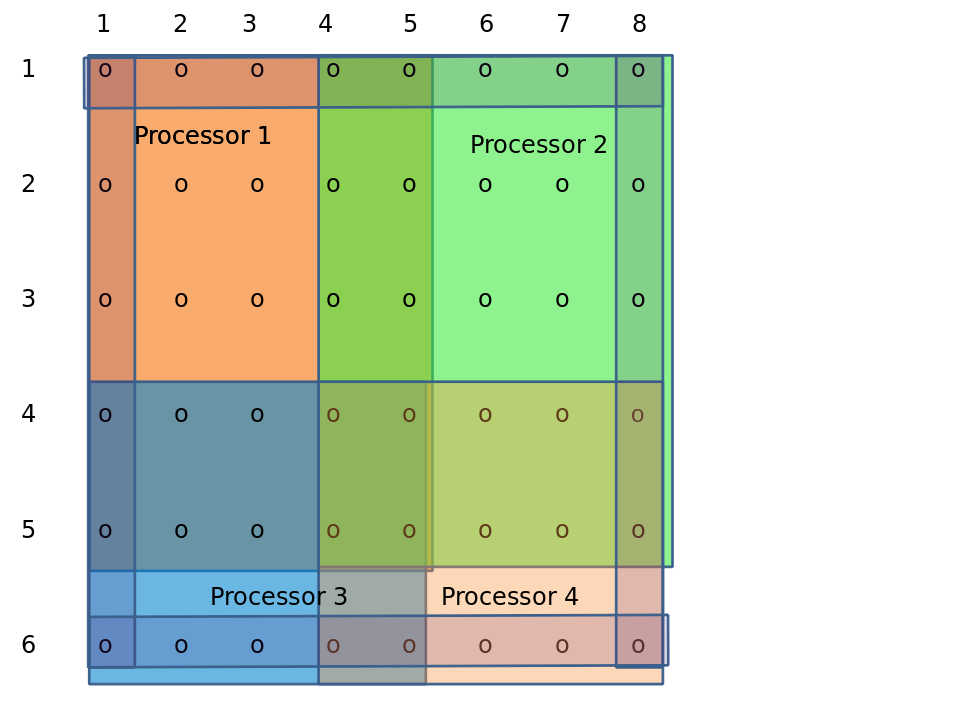
\includegraphics[width=10cm]{configuration.png}
\caption{Configuration of Processors}
\label{fig:configuration}
\end{center}
\end{figure}

Figure  \ref{fig:configuration} is an example.
In figure \ref{fig:configuration}, "o" is an element in the Psi or Omega matrix.
Row 1,6 and column 1,8 are the boundaries.
Here, we have 4 processors.
Processor 1 stores the part covered by red square
which ranges from row 1 to 5 and column 1 to 5.
Processor 2 stores the part covered by green square,which ranges from
row 1 to 5 and from column 4 to 8.
Processor 3 stores the elements covered by the blue square.
But processor 1 only calculate elements from row 2 to row 4 and from column
2 to column 4.
The rest elements are considered as the boundary of processor 1.
Although column 5 is the boundary of processor 1,  it is not the boundary
of processor 2.
So processor 2 will calculate column 5 and send the value of these elements
to processor 1. In the same way, processor 3 will calculate row 5 and send
them to processor 1.
So processor 1 will have updated value for all the elements.
For the same reason, all the processors will get the new values for the matrices
after one iteration.
The criterion to stop the iteration is the maximum difference between
the old matrix and the new matrix is smaller than a specific value PsiTol.
So when finishing an iteration, the maximum difference between the old Psi
matrix and the new Psi matrix is calculated in all the processor.
We use \texttt{MPI\_Allreduce} to gather the maximum value in different
processors and compare them with PsiTol to determine whether to continue
next iteration or not.

\section{Input}

The serial program uses a command-line dialog to query the user for
configuration parameters before starting a simulation.
This includes grid size, fluid physical parameters, simulation
time and timestep, and artificial jet specifications, if any.

In parallel, such information should not be queried through the
command line, especially for a batch job.
We developed a configuration file format to store this information.
In parallel, our program uses rank 0 to read the configuration file
and broadcast the data to other ranks.
Editing this file is also a convenient way to change parameters compared
with re-running the command line dialog.
We retain the dialog, which is accessible using the ``config" argument
when running the program, since it is a descriptive way to generate
an initial configuration.

Once a configuration is generated, a simulation can be started
by giving the program two arguments: ``run" and the name of the
configuration file.

\section{Partitioning}

The parallel operation of this program requires us to partition
the structured rectangular grid on which fields are defined.
We use a rather naive and expensive but effective partitioner.
It tries all possible partitions of a particular class
and chooses the best one.
In this case a partition is better than another partition
if it has both less maximum computation and less
total communication.
Maximum computation is the largest number of grid points given to
any process, and communication is the total number of grid points
that have to be exchanged to synchronize a field after on step
of computation.

The class of partitions we choose are those for which two integers
$p_x,p_y$ exist such that the number of processes is $p_xp_y=p$.
Each rank is assigned coordinates $(i,j)\in p_x\times p_y$.
Most ranks ($i<p_x,j<p_y$), receive a sub-grid of the global
$m\times n$ grid which is of size
$\lceil\frac{m}{p_x}\rceil\times \lceil\frac{n}{p_y}\rceil$.
The other ranks receive the remaining grid points along the top
and right of the grid.
This class of partitions has some benefits and limitations.
The main benefit is that maximum workload is well minimized.
Most ranks have the maximum workload, and only a few have less work.
The limitation is in the division process along each dimension,
e.g. not all values of $m$ and $p_x$ are valid.
In that case that all possible values of $p_x,p_y$ are incompatible with
the grid dimensions $m,n$, the partitioner fails.
This did, in fact, occur in some of our experiments.

\section{Parallel Boundary Conditions}
%Micah
For any interior point in either Psi or Omega, the value is calculated
as a function of values in matrix cells one step to the north, south, east, or
west. This is not true of the extreme boundaries of the matrix. Therefore,
calculation of boundaries requires use of both the local and global position
within the matrix. This results in greater deviation in code structure from
the serial version when calculating the boundary conditions than the interior.
For any local boundaries, a check is performed to determine whether the
local boundary is also a global boundary. For many of the boundaries
that is the only changes necessary, the value being calculated in a manner
with similar requirements to the interior. Jets and boundary layers each
introduce requirements for global position in the boundary layer.
The side boundaries involve boundary layers which depend additionally
on the side of the boundary layer where particular cell exists. Jets affect
the lower boundary, and calculations vary by whether a cell is located
before, within, or after the region of the jet. Within the jet, Psi
is determined using just the simulation time and the linear position
of the cell. However, past the end of the jet, each cell on the Psi
boundary is always equal to the value of the last cell within the jet.
This introduces a problem when this last cell is not within the local
matrix. Generally, this kind of issue is delt with by having the
owning process broadcast the value of the cell. Fortunately, values
within the jet do not depend on the values of any fields. The only
value required that is not stored locally is simply the linear position
which would have been stored in the position vector. This value can
be quickly calculated, and, as a result, the value for the jets can be
computed once locally without requiring any additionaly communication.
The only additional concern is that the lower boundary of Omega requires
values of Psi two steps into the field instead of one. This does not
actually introduce any new requirements. For this calculation to fail,
the local dimension in $Y$ would be one. Such a partitioning should
never occur as every owned row would have to be sent twice per round
of computation.

\section{Parallel File IO}

In order to easily verify our results using the serial code,
we chose to implement single-file IO.
On the other hand, we would like to get some parallelism in
file IO so that it does not cripple scaling, so we try to use
MPI's parallel file IO routines to write the file in parallel.
An additional complication is that the file is in a text format
rather than binary.
Fortunately, the file is formatted such that all values are
padded to a known character width, so the offset in characters
of every value and the total file size are easily computable.
To write our output file, we first open a file collectively
with \texttt{MPI\_File\_open} and then 
allocate enough characters for the whole output with
\texttt{MPI\_File\_preallocate}.
We use
\texttt{sprintf} to produce a text string of know length for
each floating-point value, and then use
\texttt{MPI\_File\_write\_at} to write the text string at
the correct location in the file.
Each process computes its own offsets and writes concurrently
without any synchronization until all processes close the file.
This is theoretically a scalable algorithm, although in practice
operating system and MPI limits are likely to limit scaling
to some upper bound.

\section{Results}

\verbatiminput{mpi/bigtestconfig.txt}
\verbatiminput{mpi/Bigtestconfig.txt}
\myimage{one_calc.png}{Field computation scaling for input 1}{fig:calc1}
\myimage{one_file.png}{File IO scaling for input 1}{fig:file1}
\myimage{two_calc.png}{Field computation scaling for input 2}{fig:calc2}
\myimage{two_file.png}{File IO scaling for input 2}{fig:file2}

The first thing to note is that both these critical sections exhibit
essentially perfect linear strong scaling for all cases run.
In particular, the MPI File IO implementation was able to concurrently
write to one file from thousands of processes.

\section{Future Work}

\section{Conclusions}

\section{References}

\end{document}
